%% Capitol 1

\chapter{Introducció}
Els textos d'aquest llibre es basen en les publicacions de l'autor al blog publicat durant el 2017 i 2018 (\url{https://sistemesencastats.wordpress.com}). El llibre en si està publicat com a codi obert a l'adreça \url{https://github.com/mariusmm/Llibreencastats} on es pot baixar tot el codi \LaTeX\ i generar el pdf un mateix.

Com es comenta en el propi blog, suposem que el lector té coneixements de programació en llenguatge C, coneixements bàsics d'arquitectura de computadors i nocions bàsiques d'electrònica.

Tot el codi dels exemples està publicat amb llicència oberta (GNU GPLv3) \cite{gplv3} al repositori del curs a GitHub (\url{https://github.com/mariusmm/cursembedded}).

L'estructura del curs serà una breu introducció sobre l'arquitectura del microcontrolador que usarem durant el curs, seguirem amb una descripció dels perifèrics més habituals i un codi d'exemple per cada un. A continuació es detallarà l'ús d'un Sistema Operatiu en temps real per el desenvolupament d'aplicacions complexes, es continuarà amb un capítol dedicat al test en sistemes encastats i per últim un capítol de conceptes avançats.

\section{El que aquest llibre és}
Aquest llibre és per tot aquell que amb coneixements de programació en llenguatge C, coneixements d'arquitectures de computadors, coneixements mínims de HW i electrònica vulgui endinsar-se en la programació de sistemes encastats basats en microcontroladors.

També va dirigit a aquelles persones que tenen experiència amb sistemes tipus Arduino i volen entendre i poder afegir codi o crear noves biblioteques. Tot i que no parlarem específicament d'Arduino a cap part del llibre, els coneixements genèrics serveixen per aquest sistema.

\section{El que aquest llibre no és}
Aquest llibre està pensat per donar una introducció a certs aspectes del disseny i programació de sistemes encastats basats en microcontroladors, des de l'ús de biblioteques de fabricants fins a Sistemes Operatius en Temps Real.

El que no tracta aquest llibre és de plataformes existents com ara Arduino \cite{ARDUINO}. Aquesta plataforma, tot i que molt valuosa i que ha popularitzat immensament la programació i l'ús de sistemes encastats al gran públic, gràcies sobretot a la seva senzillesa d'ús i a la enorme quantitat de codi d'exemple i biblioteques, creiem que no és adequada per donar un visió detallada de tots els temes que es volen tractar en aquest llibre. Vist d'una altra manera, l'objectiu d'aquest curs és, entre d'altres, habilitar al lector usuari d'Arduino perquè pugui desenvolupar per si mateix noves biblioteques de baix nivell d'Arduino i entendre com està implementat.

Tampoc és un tractat específic sobre l'{\em interface} amb sensors i el coneixement profund sobre el tema. Per aquest cas concret, hi ha magnífics llibres amb una descripció exhaustiva sobre el tema, com per exemple aquest \cite{SensorTechnology}.

\section{Material per seguir el curs}
Tot seguit es presenta el material necessari per fer les parts pràctiques del curs, això inclou una placa de prototipat i uns pocs components, tots ells de baix preu.

\subsection{Placa de prototipat}
La part pràctica del curs es basa en la placa de prototipat EFM32TG-STK3300 Starter Kit de Silicon Labs. Aquesta placa porta un microcontrolador EFM32TG840F32 amb 32 KB de memòria \gls{FLASH} i 4 KB de memòria \gls{RAM} (veure el Reference Manual \cite{EFM32TGRM} i més endavant \fullref{sec:cortex}).

Aquesta \gls{PCB} porta un parell de botons, un \gls{LED} i un connector on hi ha tot de pins amb diferents funcions que podrem utilitzar quan ho necessitem.

Per treballar amb aquesta plataforma, cal instal·lar el conjunt d'aplicacions {\bf Simplicity Studio} versió 4 \cite{simplicityURL}. Hi ha versions per Linux, Mac i Windows.

\begin{figure}
 \centering
 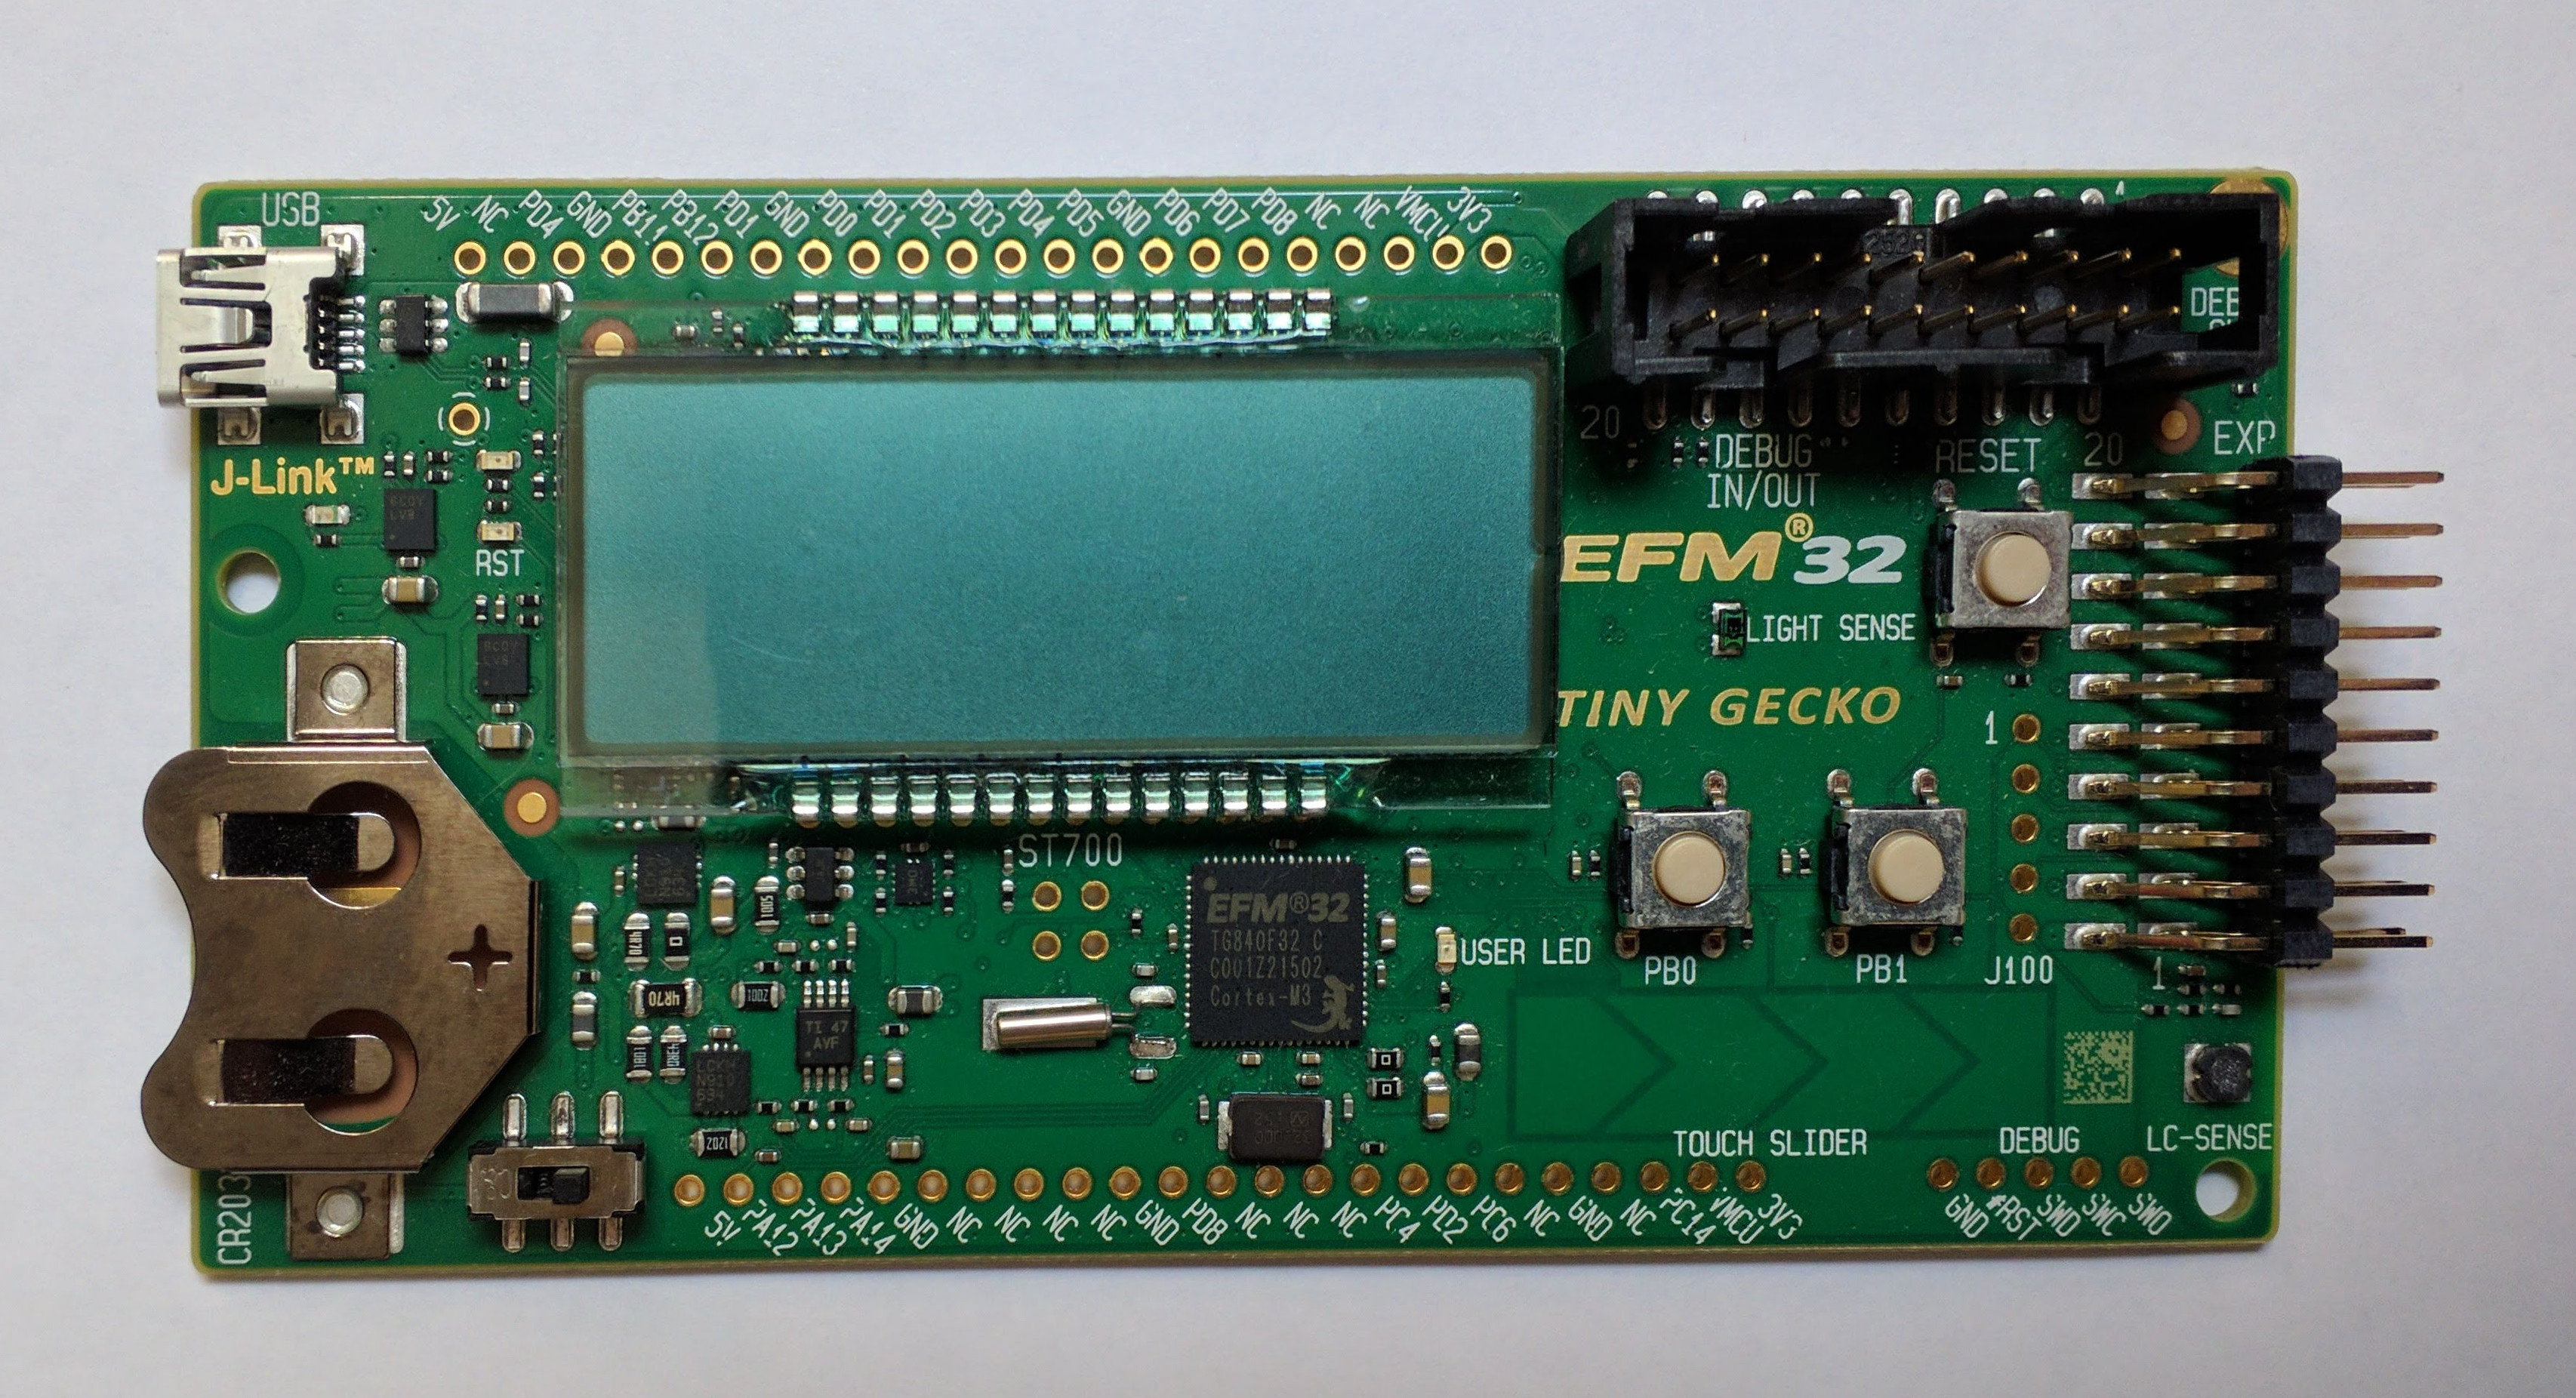
\includegraphics[width=0.85\textwidth, keepaspectratio]{imatges/tiny-gecko-starter-kit.jpg}
 \caption{Fotografia de la placa de desenvolupament de SiliconLabs}
 \label{fig:EFM32_DVK}
\end{figure}


\subsection{Dispositius auxiliars}
Per tenir dades variades i de diferent natura per les aplicacions d'exemple, farem servir els següents dispositius auxiliars:
\begin{itemize}
 \item Potenciòmetre: aquest component, que és una resistència variable, ens permetrà probar un \gls{ADC}
 \item Sensor de llum, color i moviment APDS-9960 \cite{apds9960}. Es pot adquirir a qualsevol botiga on-line ja muntat a una \gls{PCB} que incorpora uns connectors senzills per connectar-la a la PCB de desenvolupament.
 \item Cables de connexió tipus Dupont amb connector femella als dos extrems (Figura~\ref{fig:dupont}).
\end{itemize}

\begin{figure}
 \centering
 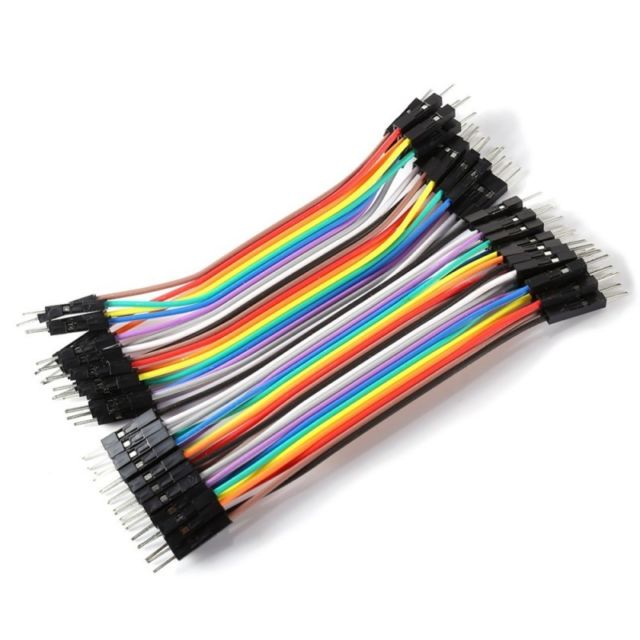
\includegraphics[width=0.45\textwidth, keepaspectratio]{imatges/cables_dupont.jpg}
 \caption{Cables dupont}
 \label{fig:dupont}
\end{figure}

\section{Eines}

Per treballar amb microcontroladors ens calen un conjunt d'eines específiques i algunes de més genèriques. Anem a veure-les amb un cert detall.

\subsection{Programadors i {\em debuggers}}
Un microcontrolador (també dit \gls{MCU} o \textmu C) es diferència d'un processador de propòsit general en moltes coses, però una de les diferències més notables és que el propi microcontrolador generalment incorpora la seva pròpia memòria (tanta \gls{RAM} com \gls{ROM}) on s'emmagatzema el codi a executar i les variables i dades a tractar. Quan el microcontrolador s'engega comença a executar el codi que troba a la ROM a certa posició.

Per descarregar el fitxer binari a la ROM, cal un dispositiu extern al microcontrolador que emmagatzema el fitxer a la ROM del microcontrolador. Aquests dispositius poden ser totalment externs al nostre circuit, i es coneixen com programadors o darrerament es veuen incorporats a la pròpia \gls{PCB} i s'hi accedeix via USB. Sigui com sigui, cal aquest programador per gravar la memòria FLASH (que funciona com una ROM pel microcontrolador).

A més, aquest programador sol afegir característiques de {\em debug}, de manera que podem controlar l'execució del microcontrolador, inspeccionar el valor de variables o posicions de memòria, accedir a la consola de {\em debug}, etc.

\subsection{{\em Toolchain}}
Com per tot processador, cal un seguit d'eines que ajudin a traduir el nostre codi (normalment C o C++) en instruccions màquina que la CPU pugui processar. Aquestes eines son el compilador i el {\em linker}. El compilador fa aquesta traducció pròpiament dita i genera fitxers objecte i el {\em linker} recull tot de fitxers objecte per crear un sol fitxer executable o biblioteca.

En el cas dels microcontroladors, hem d'acabar obtenint un fitxer executable que serà el que el microcontrolador començarà a executar quan s'engegui. Aquest fitxer haurà de tenir tot el conjunt de biblioteques i funcions necessàries per la correcta execució de l'aplicació, ja que en aquest context no tenim cap mena de sistema operatiu que ens proporcioni cap ajuda ni biblioteques.

També és habitual disposar d'algun \gls{IDE} que ens agrupa totes les eines en un entorn amigable i senzill (veure~Figura~\ref{fig:IDE}.)

\begin{figure}
 \centering
 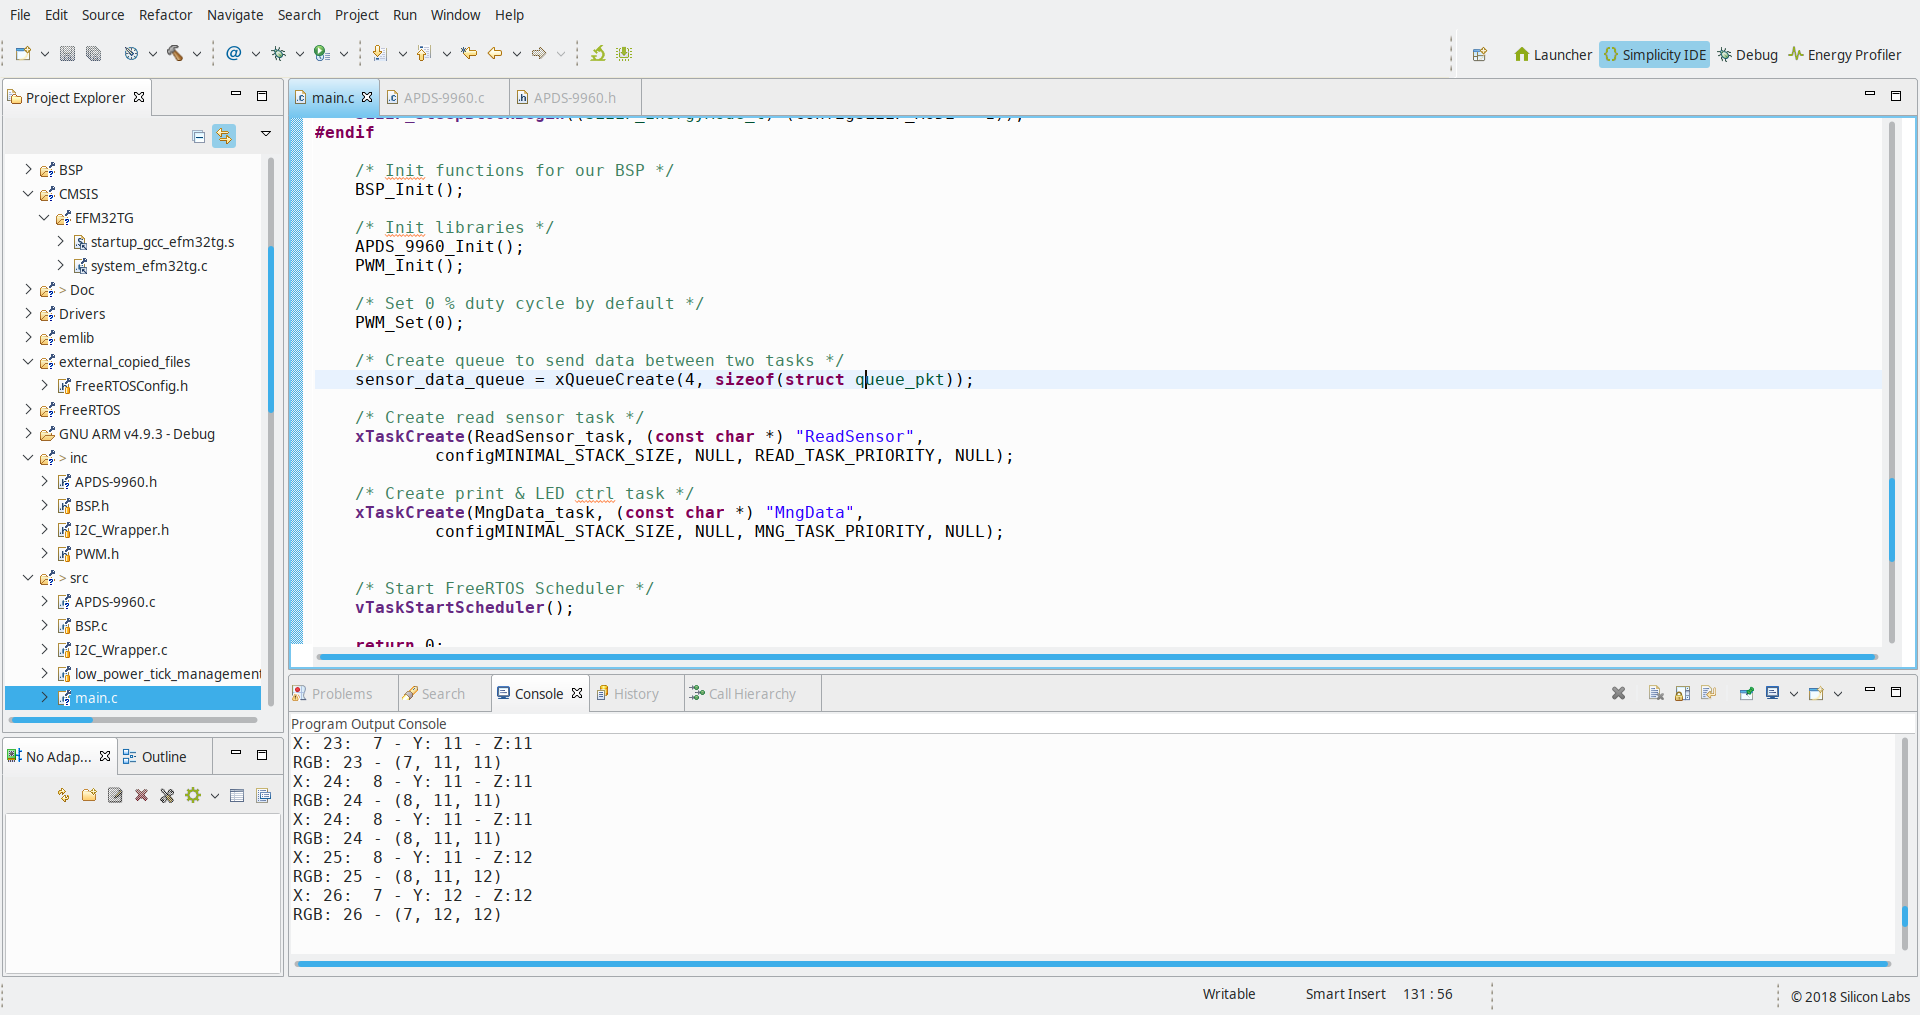
\includegraphics[width=0.85\textwidth, keepaspectratio]{imatges/capturaIDE.png}
 \caption{Aspecte del IDE Simplicity Studio\texttrademark de SiliconLabs}
 \label{fig:IDE}
\end{figure}

L'\gls{IDE} de Simplicity fa servir com a compilador el compilador per ARM de GNU \cite{ARMGNU}. Aquest compilador és de codi obert i lliure i és àmpliament utilitzant per la majoria de fabricants a les seves eines.

